\documentclass[tikz,border=3mm]{standalone}
\begin{document}
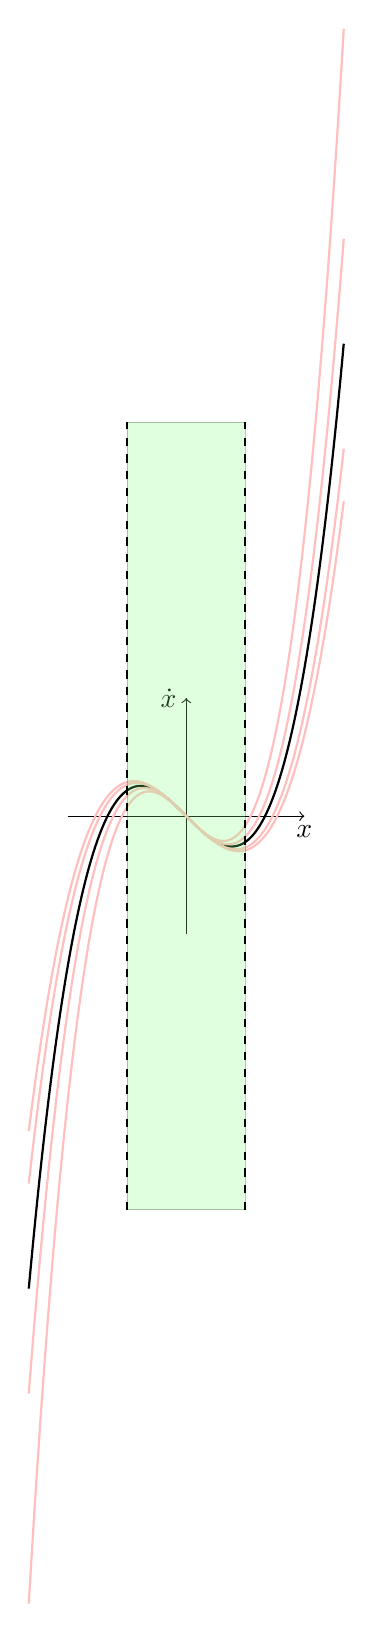
\begin{tikzpicture}[domain=-2:2,samples=400]
    \draw[->] (-1.5,0) -- (1.5,0) node[below] {$x$};
    \draw[->] (0,-1.5) -- (0,1.5) node[left] {$\dot{x}$};
    % \foreach \i in {-1,1} {
    %     \draw (\i,.1) -- (\i,-.1) node[below] {$\i$};
    % }

    % \foreach \i in {-1,1} {
    %     \draw (.1,\i) -- (-.1,\i) node[left] {$\i$};
    % }

    \draw[black, thick] plot (\x,{-\x + \x*\x*\x});

    \foreach \w in {3/4, 5/6, 7/6, 3/2} {
      \draw[pink, thick] plot(\x, {-\x + \w*\x*\x*\x});
    }

    % Fill the region of attraction
    \draw[fill=green!50, nearly transparent] (-.75,-5) -- (-.75,5) -- (.75,5) -- (.75,-5) -- cycle;

    % Draw the dashed lines around the region of attraction.
    \draw[dashed, thick, black] (-.75,-5) -- (-.75,5);
    \draw[dashed, thick, black] (.75,-5) -- (.75,5);

    % \draw[red] (-1,0) circle [radius=6pt];
    % \draw[red] (1,0) circle [radius=6pt];
    % \filldraw (0,0) circle [radius=3pt];
\end{tikzpicture}
\end{document}